\chapter{Anexo 1}
\section{Instalaci�n manual de Drupal 7}
El manual b�sico para la instalaci�n no autom�tica de Drupal es el siguiente:
\begin{enumerate}
	\item Descargar el archivo comprimido de Drupal 7 de la web https://www.drupal.org/project/drupal como se puede ver en la Figura \ref{fig:drupins1}.
	\begin{figure}
		\centering{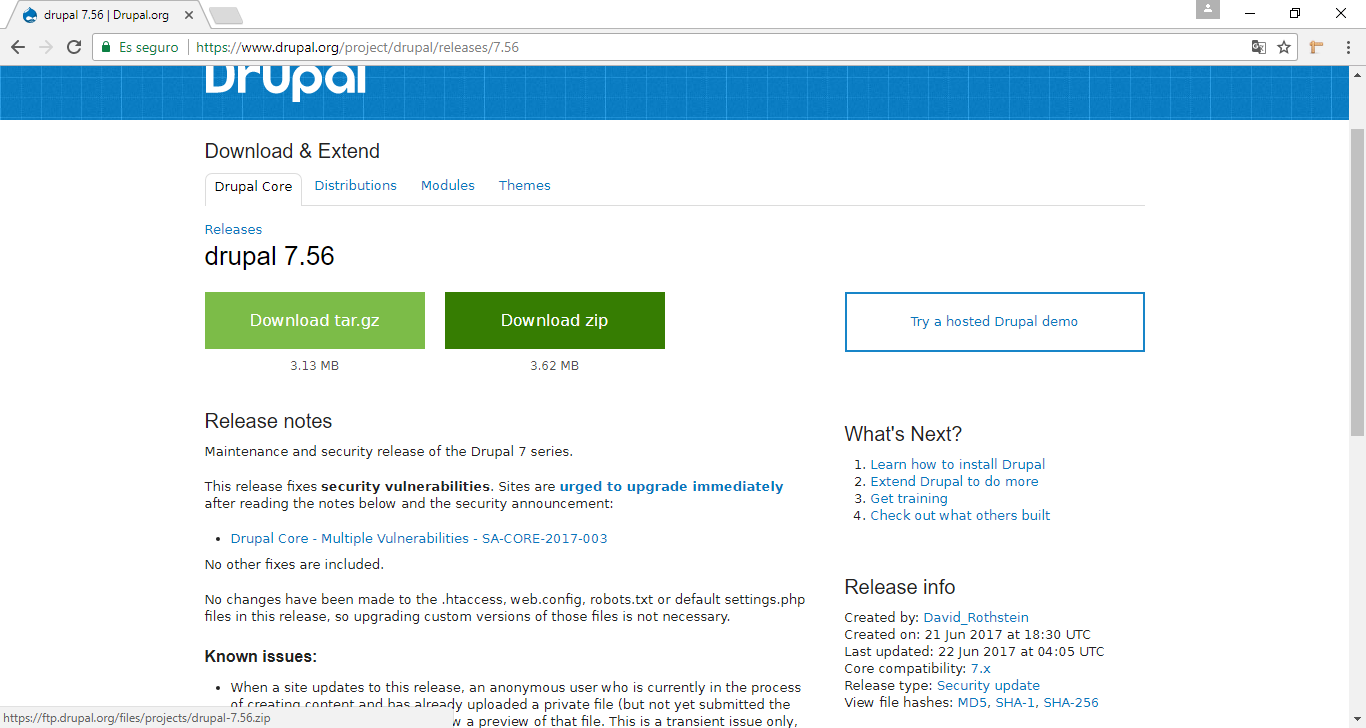
\includegraphics[width=\textwidth]{./imagenes/install_drupal_1.png}}
		\caption{Web de descarga de Drupal}
		\label{fig:drupins1}
	\end{figure}
	\item Extraer el contenido del archivo comprimido en la instalaci�n de WAMP, concretamente en la carpeta \textless instalaci�n\_de\_WAMP\textgreater /www/.
	\item Renombrar directorio de la aplicaci�n.(En el ejemplo warpdf).Figura\ref{fig:drupins2}.
	\begin{figure}
		\centering{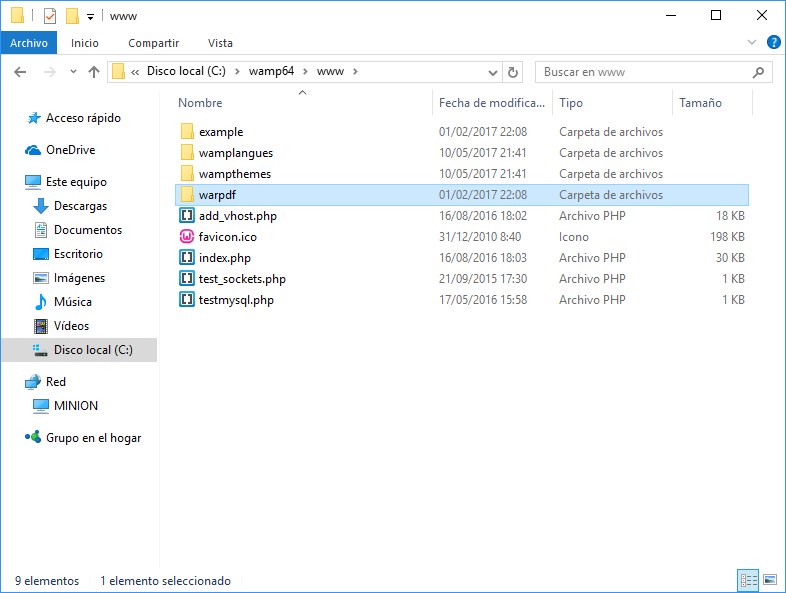
\includegraphics[width=\textwidth]{./imagenes/install_drupal_2.png}}
		\caption{Directorio de la aplicaci�n de Drupal}
		\label{fig:drupins2}
	\end{figure}
	\item Crear la base de datos en el servidor de MySQL (Depende del gestor utilizado, en el ejemplo phpMy).Figura\ref{fig:drupins3}.
	\begin{figure}
		\centering{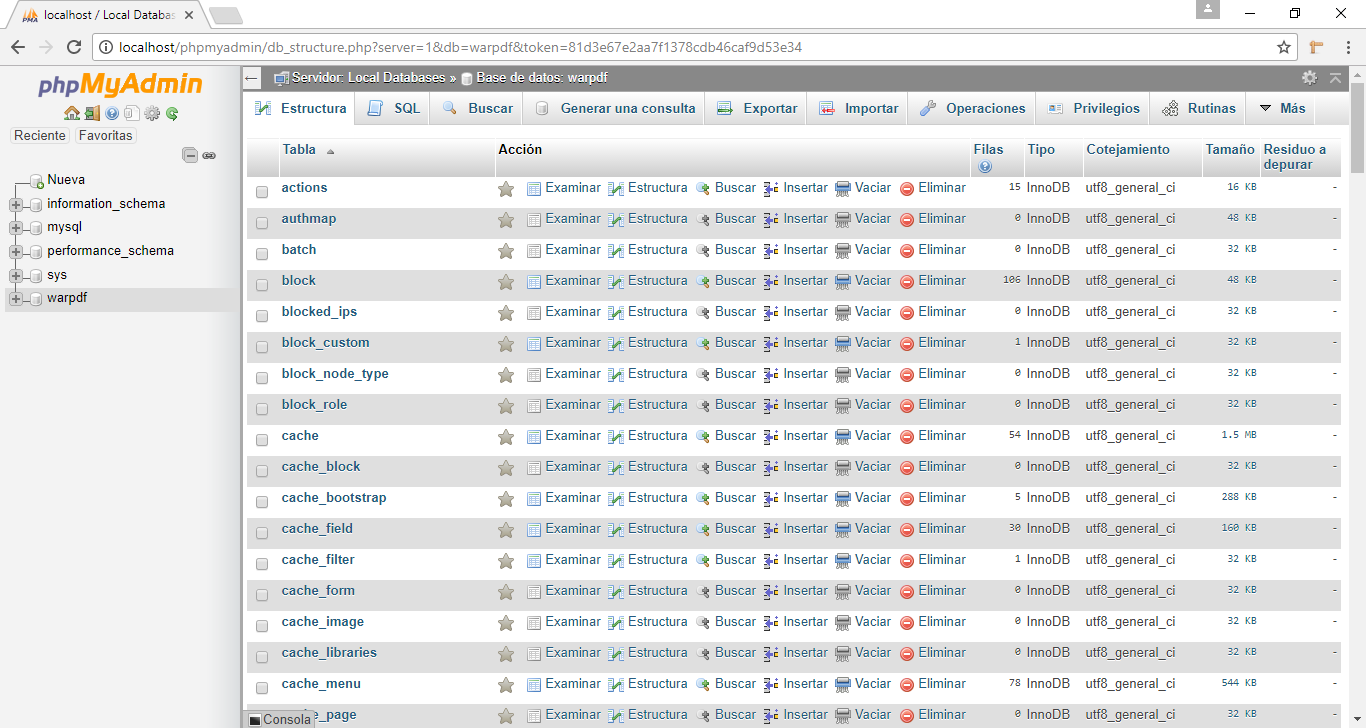
\includegraphics[width=\textwidth]{./imagenes/install_drupal_3.png}}
		\caption{Creaci�n de la base de datos}
		\label{fig:drupins3}
	\end{figure}
	\item Navegar a la aplicaci�n de Drupal desde el navegador, en el ejemplo http://localhost/warpdf.
	\item Seguir los pasos del instalador indicando que se utilice la base de datos del paso 3. Figura\ref{fig:drupins4}.
	\begin{figure}
		\centering{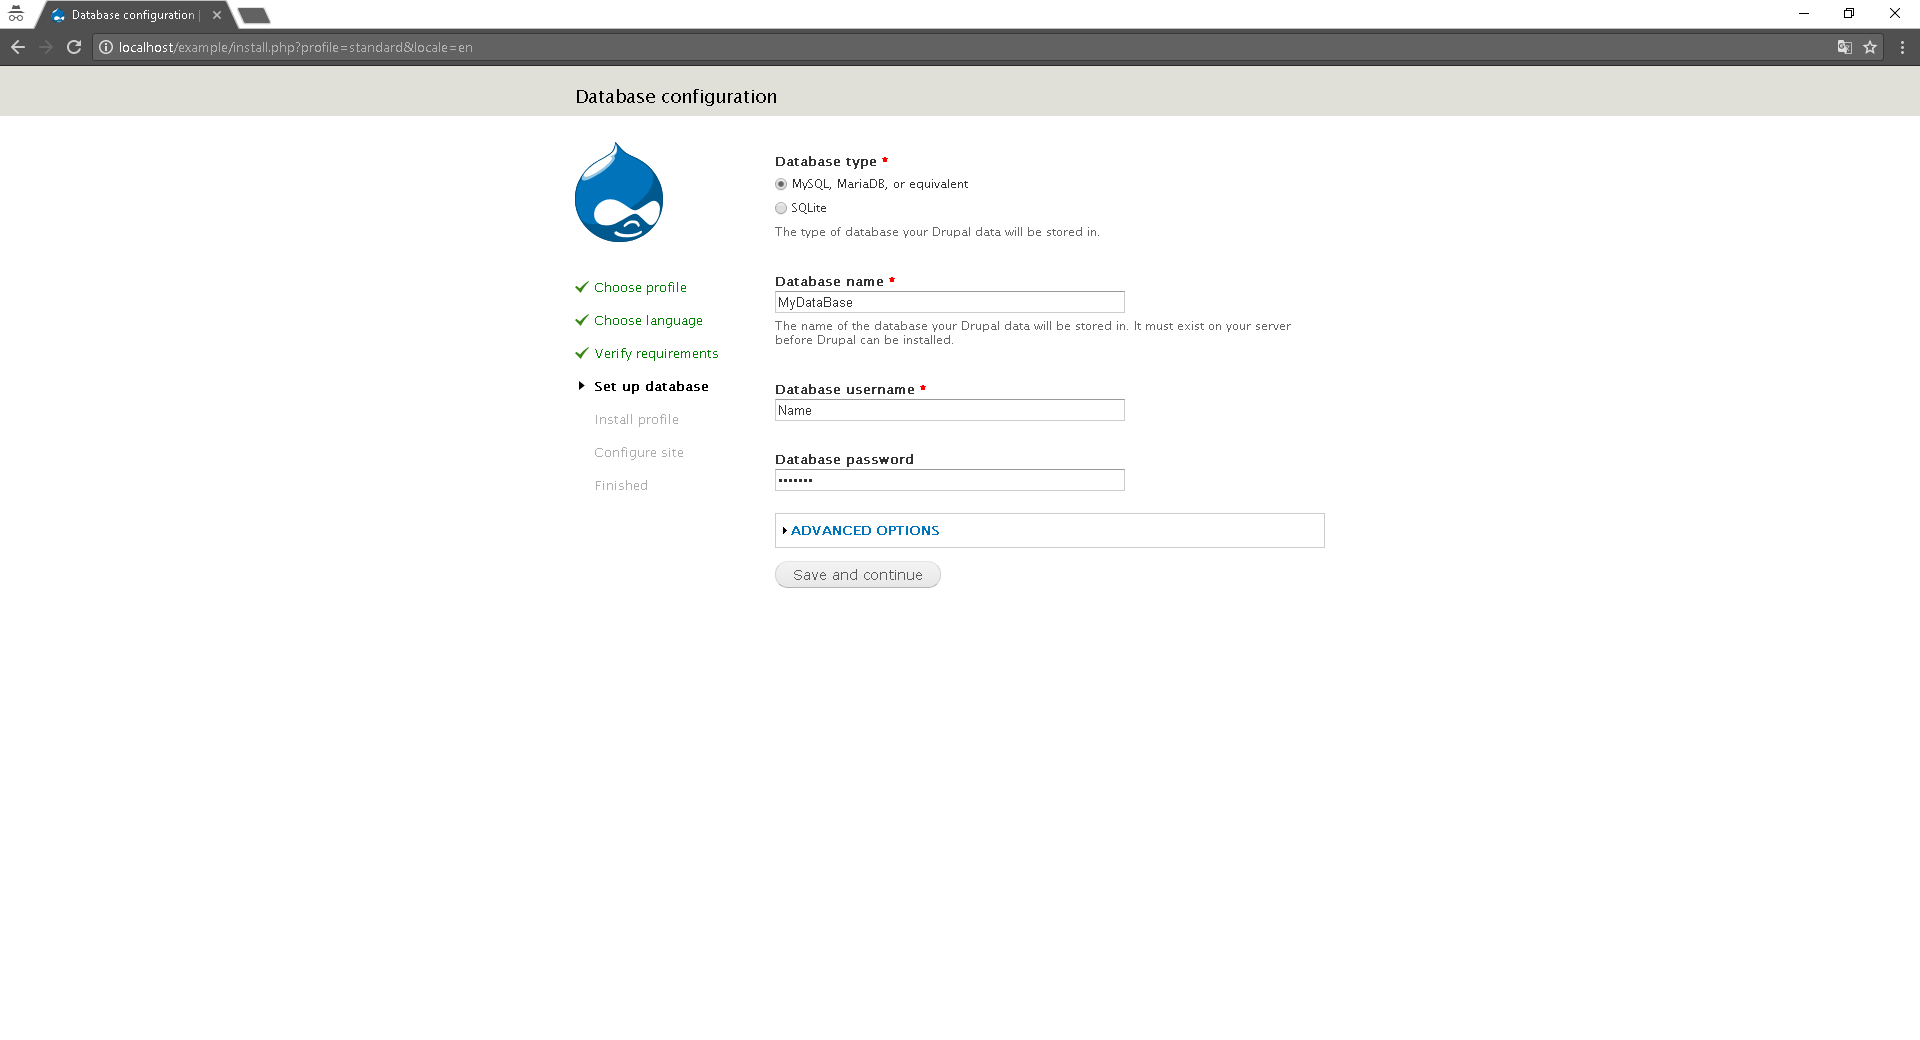
\includegraphics[width=\textwidth]{./imagenes/Wizard_drupal.png}}
		\caption{Wizard de Drupal}
		\label{fig:drupins4}
	\end{figure}
\end{enumerate}
\clearpage
\section{Manual de instalaci�n del m�dulo PDF-Warp}
Para instalar el m�dulo PDF-Warp primero se deben cumplir previamente los siguientes requisitos en la instalaci�n de Drupal:
\begin{itemize}
	\item Tener instalado y activado el m�dulo Ubercart con su m�dulo de productos y cat�logos, adem�s de sus dependencias.
	\item Tener instalado y activo el m�dulo Angularjs con la versi�n 1.6x, adem�s de sus dependencias.
	\item Tener instalado y activo el m�dulo Views Datasource, en concreto su m�dulo views\_json.
\end{itemize}
Cumpliendo estos requisitos, el manual de instalaci�n es el siguiente:
\begin{enumerate}
	\item Obtener el archivo comprimido con los componentes del m�dulo pdf\_warp.
	\item Navegar al men� ``\textit{Modules}'' dentro de la instalaci�n de Drupal.
	\item Acceder a al opci�n ``\textit{Install new Module}''.(Figura \ref{fig:pdfins1})
	\item Elegir la opci�n ``\textit{Upload a module or theme archive to install}'' buscar el archivo del m�dulo pdf\_warp y seleccionarlo.
	\item Pulsar el bot�n ``\textit{Install}''.(Figura \ref{fig:pdfins2})
	\item Activar el m�dulo desde la lista de m�dulos instalados seleccionando su \textit{checkbox} y pulsando el bot�n ``\textit{Save Configuration}''.(Figura \ref{fig:pdfins3})
\end{enumerate}

\begin{figure}
	\centering{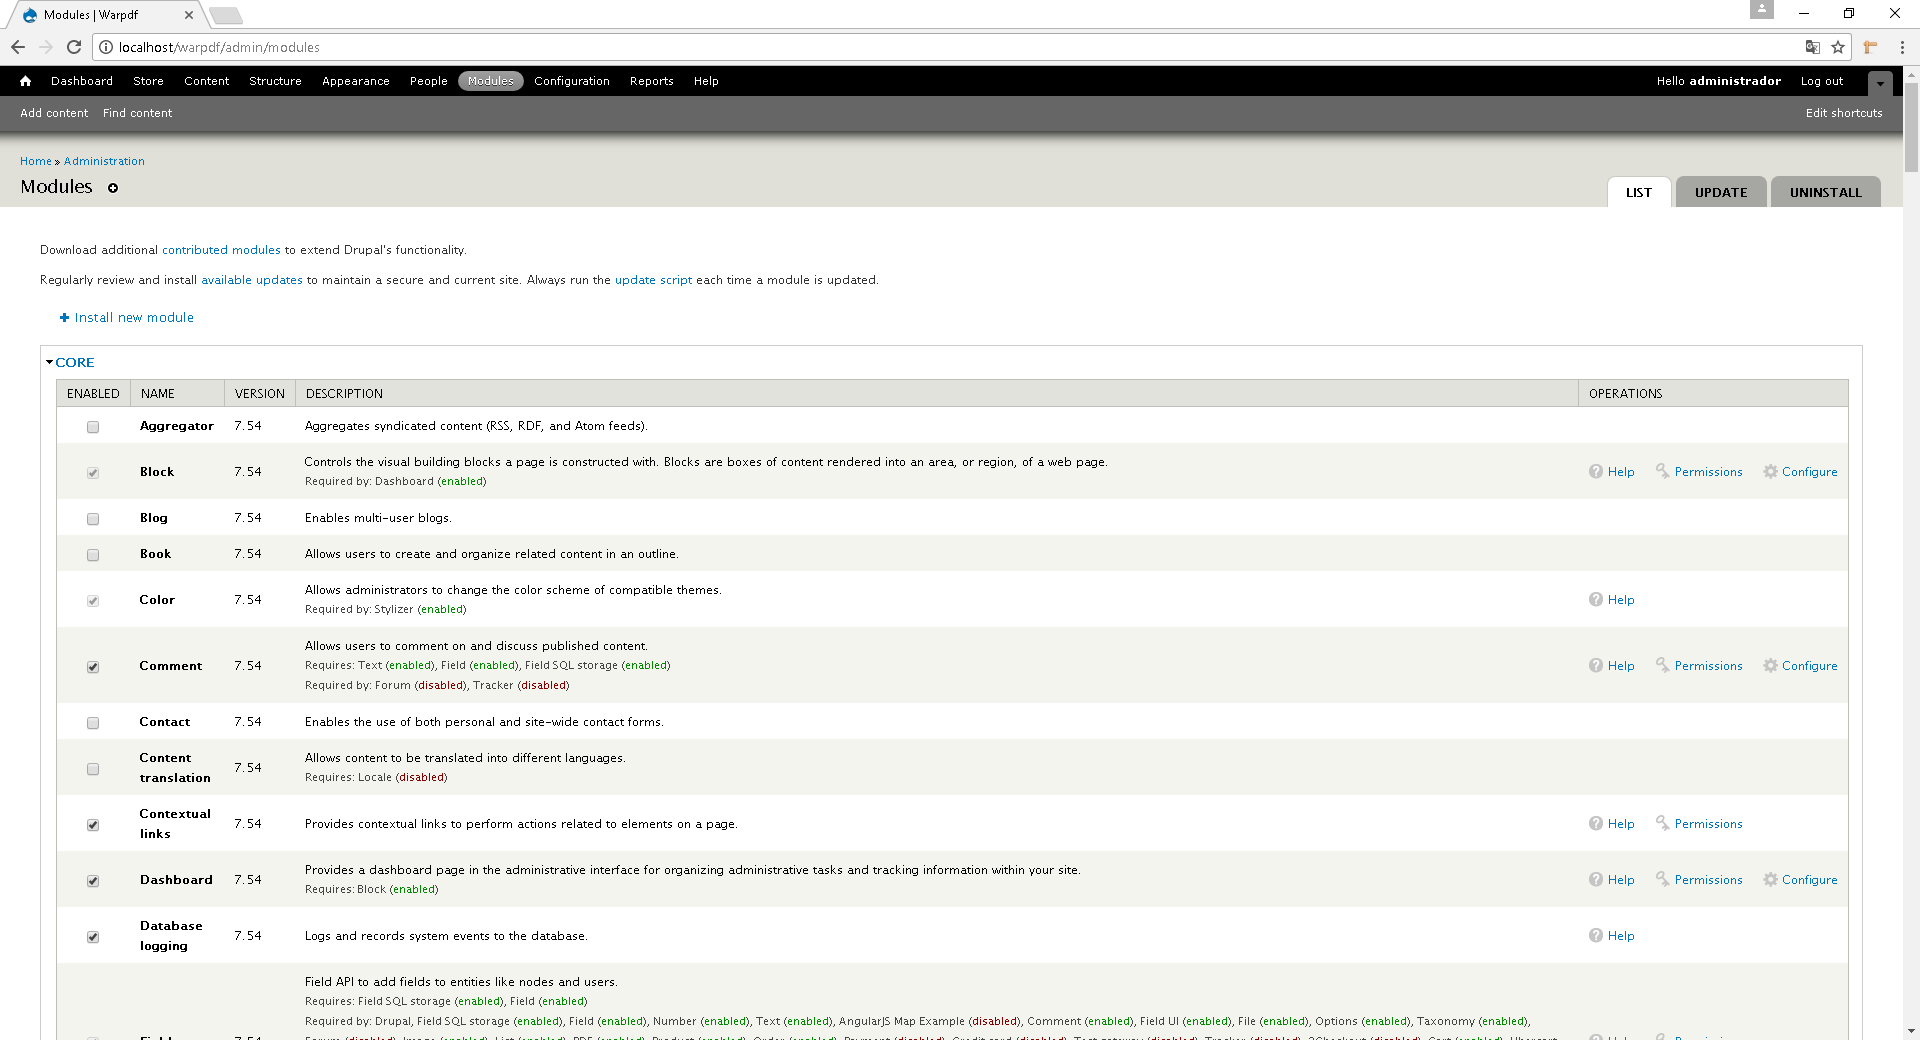
\includegraphics[width=\textwidth]{./imagenes/modules.png}}
	\caption{Lista de m�dulos y bot�n \textit{Install new module}}
	\label{fig:pdfins1}
\end{figure}
\begin{figure}
	\centering{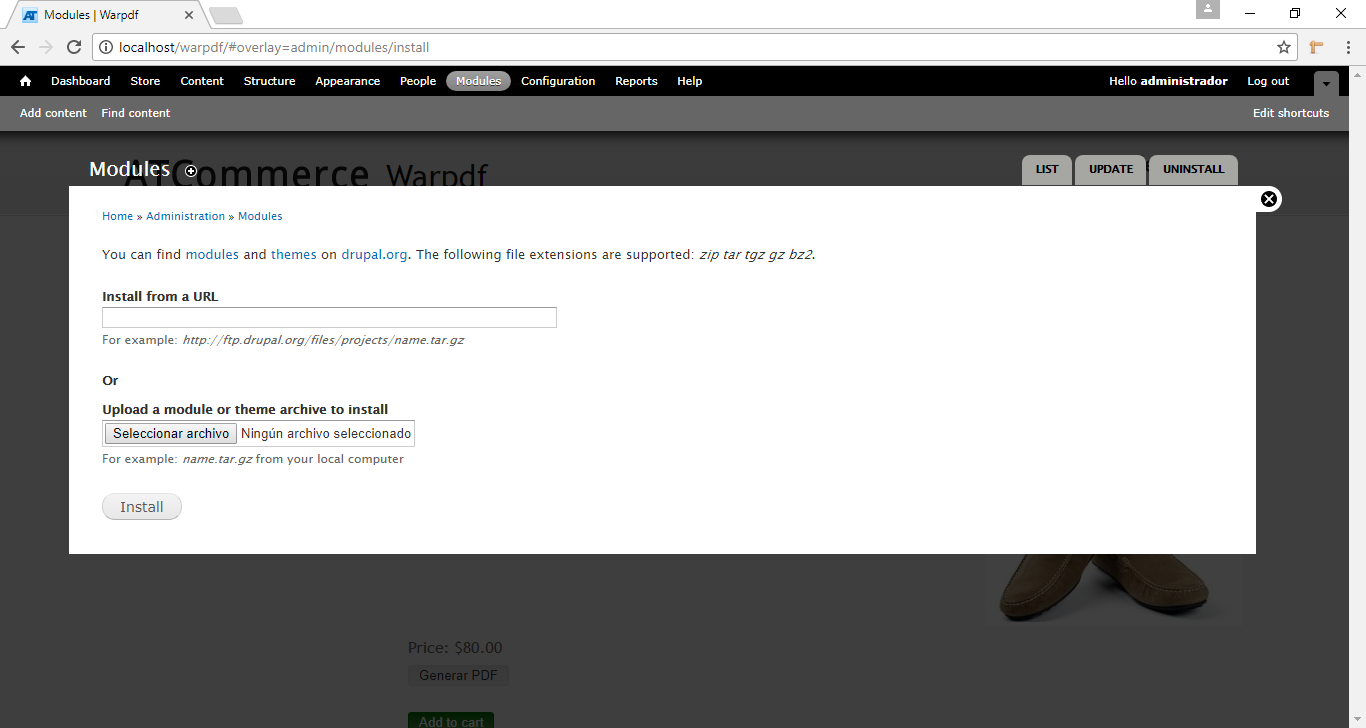
\includegraphics[width=\textwidth]{./imagenes/install_pdf_1.png}}
	\caption{Selecci�n de modo de instalaci�n de m�dulo}
	\label{fig:pdfins2}
\end{figure}
\begin{figure}
	\centering{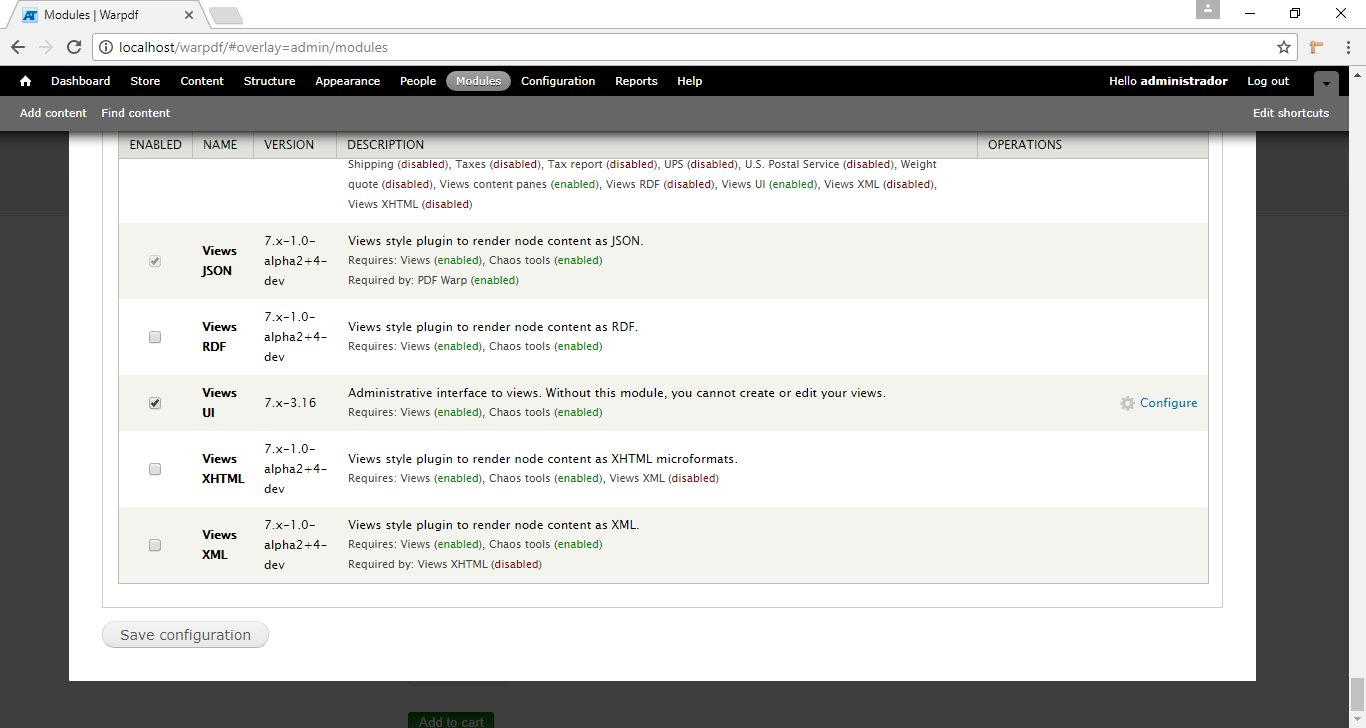
\includegraphics[width=\textwidth]{./imagenes/install_pdf_2.png}}
	\caption{Bot�n \textit{Save Configuration}}
	\label{fig:pdfins3}
\end{figure}